\documentclass[10pt,titlepage]{article}

\usepackage[american]{babel}
\usepackage[utf8]{inputenc}
\usepackage[T1]{fontenc}
\usepackage{lmodern}
\usepackage{amsmath,amsfonts,amssymb,amsthm}
\usepackage{graphicx}
\usepackage{geometry}
\geometry{a4paper}
%\usepackage{parskip}
\usepackage{graphicx}
\usepackage{epstopdf}
\usepackage{color}
\usepackage[tt]{titlepic}
\usepackage{fancyhdr}
\usepackage{enumerate}
\usepackage{lastpage}
\usepackage[labelformat=simple]{subcaption}
%\usepackage{subfigure}
\usepackage{caption}
\usepackage{bm}
\usepackage{verbatim}
%\usepackage[numbered,framed]{matlab-prettifier}
\usepackage{bigfoot}
\usepackage{afterpage}
\usepackage{mathtools}
\usepackage{float}
\usepackage{gensymb}
%\usepackage{refcheck}
%\usepackage{theoremref}
\usepackage{algpseudocode}
\usepackage{algorithm}
\usepackage{microtype}


\mathtoolsset{showonlyrefs}

\setlength\parindent{0pt}


% Custom Defines
\usepackage[comma,numbers,sort&compress]{natbib}
\bibliographystyle{plainnat}
\usepackage[pdfstartview=FitH,
            breaklinks=true,
            bookmarksopen=true,
            bookmarksnumbered=true,
            colorlinks=true,
            linkcolor=black,
            citecolor=black
            ]{hyperref}
\newcommand{\rmd}{\textrm{d}}
\newcommand{\bi}[1]{{\ensuremath{\boldsymbol{#1}}}}
\definecolor{gray}{rgb}{0.5,0.5,0.5}


\topmargin=-0.45in      %
%\evensidemargin=0in     %
\oddsidemargin=-0.1in      %
\textwidth=6.8in        %
\textheight=9.2in       %
%\headsep=0.25in         %
\headheight=30.9pt

\graphicspath{{./Figures/}}
\renewcommand\thesubfigure{(\alph{subfigure})}

\numberwithin{equation}{section}
\numberwithin{figure}{section}
\newtheorem{definition}{Definition}
\newtheorem{theorem}{Theorem}
\newtheorem{prop}{Proposition}
\newcommand{\partialdiff}[2]{\frac{\partial#1}{\partial#2}}
\newcommand{\tens}[1]{\mathcal{#1}}
\newcommand{\floor}[1]{\lfloor #1 \rfloor}
\newcommand{\norm}[1]{\left\lVert#1\right\rVert}
\newcommand{\hadamard}[2]{\mathbf{#1} \star \mathbf{#2}}
\newcommand{\kronecker}[2]{\mathbf{#1} \otimes \mathbf{#2}}
\newcommand{\khatri}[2]{\mathbf{#1} \odot \mathbf{#2}}
\newcommand{\khatriT}[2]{\mathbf{#1} \odot^T \mathbf{#2}}

\DeclareMathOperator{\myvec}{vec}
\DeclareMathOperator{\diag}{diag}
\DeclareMathOperator{\rank}{rank}

\algnewcommand\algorithmicforeach{\textbf{for each}}
\algdef{S}[FOR]{ForEach}[1]{\algorithmicforeach\ #1\ \algorithmicdo} %to define the foreach
\algnewcommand\Andd{\textbf{and} }
\renewcommand{\algorithmicrequire}{\textbf{Input:}}
\renewcommand{\algorithmicensure}{\textbf{Output:}}

\newcommand{\figref}[1]{\figurename~\ref{#1}}

\newcommand{\expnumber}[2]{{#1}\mathrm{e}{#2}}

%to keep footnotes on same page
\interfootnotelinepenalty=10000
\usepackage[flushmargin]{footmisc}



%======================= SET YOUR NAME HERE =======================================
\def\MyName{Niccolò Discacciati}

%======================= Titlepage (DO NOT MODIFY) ================================
\titlepic{
\includegraphics[width=7cm]{Figures/EPFL_Logo.eps}}
\title{\textbf{Structure exploiting Lanczos method for Hadamard product of low-rank matrices} \\[10pt] Computational Linear Algebra project}

\author{~\\[3cm]~
\begin{tabular}{rl}
%Name:&\MyName~(Sciper n. 273520)\\
Name:&\MyName\\
Sciper:& 273520\\
Date:&June 5, 2019\\
Instructors:&Stefano Massei, Lana Periša
\end{tabular}}
\date{}
%==================================================================================










\begin{document}

%========================  Header (DO NOT MODIFY) =================================
\hypersetup{pageanchor=false}
\pagestyle{fancy} \pagenumbering{arabic} \setcounter{page}{1}
\addtolength{\headheight}{\baselineskip}

%\chead{ \textit{Numerical methods in heat transfer: assignments}}
\lhead{
\includegraphics[width=45pt]{figures/EPFL_Logo.eps}}
\rhead{\MyName}
%\rfoot{\vspace{5pt}{\fontfamily{phv}\fontsize{6}{6}\selectfont \MyName{}, \thepage/\pageref{LastPage}}}
\renewcommand{\headrulewidth}{0.4pt}
\maketitle
\hypersetup{pageanchor=true}
%==================================================================================

\section{Introduction}
Given two matrices $\mathbf{A},\mathbf{B} \ \in \mathbb{R}^{m \times n}$, their Hadamard product $\mathbf{C}=\mathbf{A} \star \mathbf{B}$ is defined as the entry-wise product $c_{ij}=a_{ij}b_{ij}$ for $i=1,\dots,m=I_{1}$ and $j=1,\dots,n=I_2$. It constitutes a fundamental building block of several algorithms in scientific computing and data analysis, partly because Hadamard products of matrices correspond to products of bi-variate functions. Consider a discretization of the rectangle $\Omega=[a_1,b_1] \times [a_2,b_2]$ made by points $a_k \leq \xi_{k,1} < \cdots <  \xi_{k,I_k} \leq b_k$ with $k \in \{1,2\}$ and two functions $u,v:\Omega \rightarrow \mathbb{R}$. Assuming that the matrices $\mathbf{A}$ and $\mathbf{B}$ contain the evaluation of $u,v$ on the grid points, then $\mathbf{C}$ contains the evaluation of the product $uv$ on the same points.
It is known that the degree of smoothness of the underlying function is related to the low-rank approximation properties of the matrix \cite{Schneider}. In particular, if $u,v$ are sufficiently smooth, the corresponding matrices admit a meaningful low-rank approximation. The Hadamard product can also be efficiently compressed, due to regularity of $uv$. However, on the algebraic side, the element-wise product of low-rank matrices generally increases ranks, impacting negatively on the approximation properties. Despite this unfavorable aspect, exploiting the structure of the entry-wise product allows us to create fast matrix-vector multiplications, which turn out to be helpful in designing computationally efficient algorithms to construct low-rank approximations of the Hadamard product. \\
In this project we want to investigate the low-rank compression properties of the entry-wise product, aiming to construct a powerful technique to compress the resulting matrix. Particular emphasis is given to an analysis of the computational performance of the method. Note that most of the methods we present can be extended to dimensions greater than two, where matrices are suitably replaced by tensors. See \cite{Perisa} for the details.

\section{Methods}
\subsection{Definitions and properties}
In this report, matrices are denoted with boldface capital letters, while boldface lowercase letters are used for vectors, unless stated otherwise. Given a matrix $\mathbf{A}$, its columns are denoted with boldface lowercase letters, i.e. $\mathbf{A}=(\mathbf{a}_1 \cdots \mathbf{a}_n)$, while for single entries we use $\mathbf{A}_{ij}$ or $a_{ij}$\footnote{Even though the notation $\mathbf{A}_{ij}$ is more general, we often use $a_{ij}$ to ease the readability. To denote the elements of a matrix resulting from an operation, we always use the first notation, e.g., $(\mathbf{A} \ op \ \mathbf{B})_{ij}$. A similar reasoning holds for vectors.}. \\
Let ${ \myvec:\mathbb{R}^{m \times n} \rightarrow \mathbb{R}^{mn} }$ be the standard vectorization of a matrix, obtained from stacking its columns, i.e.
\begin{equation}
	(\myvec{\mathbf{A}})_i=a_{(i-1) \% m+1,\floor{(i-1)/m}+1}, \quad \text{or} \quad \myvec{\mathbf{A}}=(\mathbf{a}_1^T \ \cdots \ \mathbf{a}_n^T)^T.
\end{equation}
Moreover, for a square matrix $\mathbf{A}$, $\diag(\mathbf{A})$ denotes the vector consisting of its diagonal elements, while for a vector $\mathbf{v}$, $\diag(\mathbf{v})$ denotes a diagonal matrix with the given vector on the diagonal, i.e.
\begin{align}
	(\diag(\mathbf{A}))_i &= a_{ii}, \\
	(\diag(\mathbf{v}))_{ij} &= v_i \delta_{ij}.
\end{align}
In this work, we use the following definitions and properties.
\begin{itemize}
\item \textit{Hadamard product}. 
	Given $\mathbf{A},\mathbf{B} \in \mathbb{R}^{m \times n}$, the Hadamard or element-wise product is defined as
	\begin{equation}
	(\mathbf{A} \star \mathbf{B})_{ij}=a_{ij} b_{ij},
	\label{eqn:hadamard}
	\end{equation}
	i.e.
	\begin{equation}
	\mathbf{A} \star \mathbf{B}=
	\begin{pmatrix}
	a_{11} b_{11} & \cdots & a_{1n}b_{1n} \\ \vdots & \ddots & \vdots \\ a_{m1}b_{m1} & \cdots & a_{mn}b_{mn}
	\end{pmatrix},
	\label{eqn:hadamard_mat}
	\end{equation}
	and it is an element of $\mathbb{R}^{m \times n}$.
\item \textit{Kronecker product}. 
	Given $\mathbf{A} \in \mathbb{R}^{m \times n}$, $\mathbf{B} \in \mathbb{R}^{p \times q}$, the Kronecker product is defined as
	\begin{equation}
	(\mathbf{A} \otimes \mathbf{B})_{ij}=a_{\floor{(i-1)/p}+1,\floor{(j-1)/q}+1} b_{(i-1) \% p+1,(j-1) \% q+1},
	\label{eqn:kronecker}
	\end{equation}
	i.e.
	\begin{equation}
	\mathbf{A} \otimes \mathbf{B}=
	\begin{pmatrix}
	a_{11} \mathbf{B} & \cdots & a_{1n}\mathbf{B} \\ \vdots & \ddots & \vdots \\ a_{m1}\mathbf{B} & \cdots & a_{mn}\mathbf{B} 
	\end{pmatrix},
	\label{eqn:kronecker_mat}
	\end{equation}
	and it is an element of $\mathbb{R}^{mp \times nq}$.
\item \textit{Khatri-Rao product}. 
	Given $\mathbf{A} \in \mathbb{R}^{m \times n}$, $\mathbf{B} \in \mathbb{R}^{p \times n}$, the Khatri-Rao product is defined as
	\begin{equation}
	(\mathbf{A} \odot \mathbf{B})_{ij}=(\mathbf{a}_{j} \otimes \mathbf{b}_{j})_i= a_{\floor{(i-1)/p}+1,j} b_{(i-1) \% p+1,j},
	\label{eqn:khatri}
	\end{equation}
	i.e.
	\begin{equation}
	\mathbf{A} \odot \mathbf{B}=
	\begin{pmatrix}
	\mathbf{a}_{1} \otimes \mathbf{b}_{1} & \cdots & \mathbf{a}_{n} \otimes \mathbf{b}_{n}
	\end{pmatrix},
	\label{eqn:khatri_mat}
	\end{equation}
	and it is an element of $\mathbb{R}^{mp \times n}$.
\item \textit{Transpose Khatri-Rao product}. 
	Given $\mathbf{A} \in \mathbb{R}^{m \times n}$, $\mathbf{B} \in \mathbb{R}^{m \times q}$, the transpose Khatri-Rao product is defined as
	\begin{equation}
	\mathbf{A} \odot^T \mathbf{B}=(\mathbf{A}^T \odot \mathbf{B}^T)^T,
	\label{eqn:khatriT}
	\end{equation}
	and it is an element of $\mathbb{R}^{m \times nq}$.
\end{itemize}

\begin{prop}
	Let $\mathbf{A},\mathbf{B}$ two matrices and $\mathbf{v}$ a vector for which the required operations are well defined. Then the following properties hold:
	\begin{itemize}
		\item Property 1:
		\begin{equation}
		(\mathbf{A} \otimes \mathbf{B})\mathbf{v}=\myvec(\mathbf{B} \mathbf{V} \mathbf{A}^T), \text{ where } \mathbf{v}=\myvec(\mathbf{V}).
		\label{eqn:prop1}
		\end{equation}
		\item Property 2:
		\begin{equation}
		(\mathbf{A} \odot \mathbf{B})\mathbf{v}=\myvec (\mathbf{B} \diag(\mathbf{v}) \mathbf{A}^T).
		\label{eqn:prop2}
		\end{equation}
		\item Property 3:
		\begin{equation}
		(\mathbf{A} \odot^T \mathbf{B})\mathbf{v}=\diag (\mathbf{B} \mathbf{V} \mathbf{A}^T), \text{ where } \mathbf{v}=\myvec(\mathbf{V}). 
		\label{eqn:prop3}
		\end{equation}
		\item Property 4:
		\begin{equation}
		(\mathbf{A} \otimes \mathbf{B})^T=\mathbf{A}^T \otimes \mathbf{B}^T.
		\label{eqn:prop4}
		\end{equation}
	\end{itemize}
\end{prop}
These properties can be verified by applying the definitions of the operators, and the proof is omitted for the sake of brevity.


\subsection{A first result}
Given two matrices with low-rank structures, we want to study how the compression properties are inherited by their element-wise product. The first step aims to construct a suitable representation of the Hadamard product, starting from two matrices in a low-rank revealing format.
Hence, we let $\mathbf{A},\mathbf{B} \in \mathbb{R}^{m\times n}$ be two matrices with low-rank structures
\begin{equation}
	\mathbf{A}=\mathbf{U}_A\mathbf{\Sigma}_A\mathbf{V}_A^T, \quad \mathbf{B}=\mathbf{U}_B\mathbf{\Sigma}_B\mathbf{V}_B^T,
	\label{eqn:LR_AB}
\end{equation}
with $\mathbf{U}_A \in \mathbb{R}^{m \times k_A}$, $\mathbf{\Sigma}_A \in \mathbb{R}^{k_A \times k_A}$, $\mathbf{V}_A \in \mathbb{R}^{n \times k_B}$, $\mathbf{U}_B \in \mathbb{R}^{m \times k_B}$, $\mathbf{\Sigma}_B \in \mathbb{R}^{k_B \times k_B}$, $\mathbf{V}_B \in \mathbb{R}^{n \times k_B}$, for some $k_A,k_B \ll \min\left\lbrace m,n \right\rbrace$. Such approximations can be computed in multiple ways, with a popular technique relying on the singular value decomposition (SVD) and
\begin{theorem}[Eckart-Young \cite{Simon}]
	Let $\mathbf{A} \in \mathbb{R}^{m \times n}$ be given. Let its SVD be $\mathbf{A}=\mathbf{U} \mathbf{\Sigma} \mathbf{V}^T$ with singular values $\left\lbrace \sigma_i \right\rbrace_{i=1}^{\min\left\lbrace m,n \right\rbrace}$ in descending order. Set $\mathbf{A}_j = \mathbf{U}_j \mathbf{\Sigma}_j \mathbf{V}_j$, where $\mathbf{\Sigma}_j=\diag(\{ \sigma_1,\dots,\sigma_j \}) $, and $\mathbf{U}_j,\mathbf{V}_j$ are formed by the first $j$ columns of $\mathbf{U},\mathbf{V}$. Then
	\begin{equation}
		\left( \sum_{i=j+1}^{\min\left\lbrace m,n \right\rbrace} \sigma_i^2 \right)^{1/2}= \norm{\mathbf{A}-\mathbf{A}_j}_F=
		\min \left\lbrace \norm{\mathbf{A}-\mathbf{B}}_F | \rank(\mathbf{B})\leq j \right\rbrace.
	\end{equation}
	\label{thm:SVD}
\end{theorem}
Thus, the SVD constitutes an important tool in compression theory. In particular, \eqref{eqn:LR_AB} can be computed from the SVD, truncating the smallest singular values and the corresponding left and right vectors. \\
The Hadamard product admits a meaningful representation, as stated in the following
\begin{prop}
	Let $\mathbf{A},\mathbf{B}$ be two matrices having the structure \eqref{eqn:LR_AB}. Then
	\begin{equation}
		\hadamard{A}{B}=
		\left( \mathbf{U}_A^T \odot \mathbf{U}_B^T \right)^T
		\left( \mathbf{\Sigma}_A \otimes \mathbf{\Sigma}_B \right)
		\left( \mathbf{V}_A^T \odot \mathbf{V}_B^T \right),
		\label{eqn:LR_C}
	\end{equation}
	or, equivalently,
	\begin{equation}
	\hadamard{A}{B}=
	\left( \mathbf{U}_A \odot^T \mathbf{U}_B \right)
	\left( \mathbf{\Sigma}_A \otimes \mathbf{\Sigma}_B \right)
	\left( \mathbf{V}_A \odot^T \mathbf{V}_B \right)^T.
	\label{eqn:LR_C2}
	\end{equation}
\end{prop}
\begin{proof}
	The proof follows directly from definitions of the involved operators. The $(i,j)$ component of the left-hand-side of \eqref{eqn:LR_C} can be written as
	\begin{equation}
		a_{ij}b_{ij}=\sum_{r=1}^{k_A} \sum_{x=1}^{k_A} u^A_{ir}\sigma^A_{rx}v^A_{jx} \ \sum_{s=1}^{k_B} \sum_{y=1}^{k_B} u^B_{is}\sigma^B_{sy}v^B_{jy} =
		\sum_{r=1}^{k_A} \sum_{x=1}^{k_A} \sum_{s=1}^{k_B} \sum_{y=1}^{k_B} u^A_{ir}\sigma^A_{rx}v^A_{jx} u^B_{is}\sigma^B_{sy}v^B_{jy}.
		\label{eqn:LHS}
	\end{equation}
	The $(i,j)$ component of the right-hand-side of \eqref{eqn:LR_C} is
	\begin{align}
	&\sum_{k=1}^{k_A k_B} \sum_{l=1}^{k_A k_B} \left( \mathbf{U}_A^T \odot \mathbf{U}_B^T \right)^T_{ik} \left( \mathbf{\Sigma}_A \otimes \mathbf{\Sigma}_B \right)_{kl} \left( \mathbf{V}_A^T \odot \mathbf{V}_B^T \right)_{lj} \\
	\begin{split}
	= \sum_{k=1}^{k_A k_B} \sum_{l=1}^{k_A k_B}
	u^A_{i,\floor{(k-1)/k_B}+1} u^B_{i,(k-1) \% k_B+1}
	\sigma^A_{\floor{(k-1)/k_B}+1,\floor{(l-1)/k_B}+1} \\ 
	\sigma^B_{(k-1) \% k_B+1,(l-1) \% k_B+1}
	v^A_{j,\floor{(l-1)/k_B}+1} v^B_{j,(l-1) \% k_B+1}.
	\end{split}
	\label{eqn:sum_long}
	\end{align}
	Setting $k=(r-1)k_B+s$, $l=(x-1)k_B+y$, \eqref{eqn:sum_long} simplifies to
	\begin{equation}
		\sum_{r=1}^{k_A} \sum_{s=1}^{k_B} \sum_{x=1}^{k_A} \sum_{y=1}^{k_B} u^A_{ir}u^B_{is} \sigma^A_{rx} \sigma^B_{sy} v^A_{jx} v^B_{jy},
	\end{equation}
	which is exactly the expression \eqref{eqn:LHS}. The representation \eqref{eqn:LR_C2} follows from the definition of the transpose Khatri-Rao product \eqref{eqn:khatriT}.
\end{proof}

\subsection{Fast matrix-vector multiplications} \label{sec:matvec_hadamard}
As shown in the following Sections, the representation \eqref{eqn:LR_C} does not capture the low-rank properties of the Hadamard product. In \eqref{eqn:LR_AB}, the ranks of $\mathbf{A}$ and $\mathbf{B}$ are captured by the matrices $\mathbf{\Sigma}_A$ and $\mathbf{\Sigma}_B$ respectively, and are at most $k_A$ and $k_B$. According to \eqref{eqn:LR_C}, the rank of the Hadamard product is captured by $\mathbf{\Sigma}_A \otimes \mathbf{\Sigma}_B$, and can be up to $k_A k_B$. Thus, the ranks of $\mathbf{A}$ and $\mathbf{B}$ are (in general) multiplied, and the good compression properties of $\hadamard{A}{B}$ can be lost. Hence, this \textit{curse of dimensionality} should be avoided in order to efficiently compress the Hadamard product. 
\\
However, \eqref{eqn:LR_C} is helpful to compute efficient multiplications between the Hadamard product $\hadamard{A}{B}$ and a vector $\mathbf{v}$. Such a procedure, that avoids the explicit construction of the matrix $\hadamard{A}{B}$, can be divided in three steps.
\begin{itemize}
	\item \textit{Step 1.} Compute $\mathbf{w}_1=\left( \mathbf{V}_A^T \odot \mathbf{V}_B^T \right) \mathbf{v}$. \\
	From \eqref{eqn:prop2} we have that
	$\mathbf{w}_1=\myvec (\mathbf{V}_B^T \diag(\mathbf{v}) \mathbf{V}_A) $. In this context it is enough to compute the matrix $\mathbf{W}_1$, obtained by reshaping $\mathbf{w}_1$ into a $k_B \times k_A$ matrix. Since
	\begin{equation}
		\mathbf{w}_1=\myvec\mathbf{W}_1,
		\label{eqn:w1}
	\end{equation}
	we have
	\begin{equation}
		\mathbf{W}_1=\mathbf{V}_B^T \diag(\mathbf{v}) \mathbf{V}_A.
	\end{equation}
	The computational cost of this step is $\mathcal{O}(n k_A k_B)$, since it consists of the multiplication of the matrices $\mathbf{V}_B^T \in \mathbb{R}^{k_B \times n}$ and $\diag(\mathbf{v}) \mathbf{V}_A \in \mathbb{R}^{n \times k_A}$. Note that the product of a diagonal and a full matrix can be computed efficiently at a cost that is negligible in this framework.
	
	\item \textit{Step 2.} Compute $\mathbf{w}_2=\left( \mathbf{\Sigma}_A \otimes \mathbf{\Sigma}_B \right) \mathbf{w}_1$. \\
	Using \eqref{eqn:prop1} and \eqref{eqn:w1}, we have that
	\begin{equation}
		\mathbf{w}_2=\myvec( \mathbf{\Sigma}_B \mathbf{W}_1 \mathbf{\Sigma}_A^T ).
	\end{equation}
	Similarly to Step 1, we set
	\begin{equation}
	\mathbf{w}_2=\myvec\mathbf{W}_2.
	\label{eqn:w2}
	\end{equation}
	so that
	\begin{equation}
	\mathbf{W}_2=\mathbf{\Sigma}_B^T \mathbf{W}_1 \mathbf{\Sigma}_A^T.
	\end{equation}
	Since two matrix-matrix multiplications are performed, the cost at most of order $\mathcal{O}(k_Bk_A^2+k_Ak_B^2)$.
	
	\item \textit{Step 3.} Compute $\mathbf{w}_3=\left( \mathbf{U}_A^T \odot \mathbf{U}_B^T \right)^T \mathbf{w}_2=\left( \mathbf{U}_A \odot^T \mathbf{U}_B \right) \mathbf{w}_2$. \\
	Using \eqref{eqn:prop3} and \eqref{eqn:w2}, we have that
	\begin{equation}
	\mathbf{w}_3=\diag( \mathbf{U}_B \mathbf{W}_2 \mathbf{U}_A^T ).
	\end{equation}
	Since two matrix-vector multiplications are performed, the cost should scale quadratically with $m$. Exploiting the fact that only the diagonal elements are needed, the computational effort reduces to a multiplication between $\mathbf{W}_2 \in \mathbb{R}^{k_B \times k_A}$ and $\mathbf{U}_A^T \in \mathbb{R}^{k_A \times m}$ and it is of order $\mathcal{O}(k_A k_B m)$.
\end{itemize}
Hence, we are able to compute a matrix-vector multiplication in
\begin{equation}
	\mathcal{C}_1=\mathcal{O}(n k_A k_B + k_Bk_A^2+k_Ak_B^2 + k_A k_B m), 
\end{equation}
in comparison with
\begin{equation}
	\mathcal{C}_2=\mathcal{O}(mn),
\end{equation}
if the standard implementation is considered. If the low-rank approximations are efficiently performed, a clear speedup is present. Assuming that $m=n$ and $k_A=k_B=k$, the two costs reduce to $\mathcal{C}_1=\mathcal{O}(nk^2+k^3)$ and $\mathcal{C}_2=\mathcal{O}(n^2)$ respectively, and our implementation is preferred over the standard one when $k^2<n$, at least asymptotically. \\
Even though the procedure has been described to compute $(\hadamard{A}{B}) \mathbf{v}$, the same algorithm can be exploited to compute $(\hadamard{A}{B})^T \mathbf{w}$. From \eqref{eqn:LR_C} and \eqref{eqn:prop4}, we have 
\begin{equation}
(\hadamard{A}{B})^T=
\left( \mathbf{V}_A^T \odot \mathbf{V}_B^T \right)^T
\left( \mathbf{\Sigma}_A^T \otimes \mathbf{\Sigma}_B^T \right)
\left( \mathbf{U}_A^T \odot \mathbf{U}_B^T \right),
\label{eqn:LR_Ct}
\end{equation}
so that the previous reasoning can be applied with the following substitutions
\begin{equation}
	\mathbf{U}_A \leftarrow \mathbf{V}_A, \ \mathbf{\Sigma}_A \leftarrow \mathbf{\Sigma}_A^T, \ \mathbf{V}_A \leftarrow \mathbf{U}_A, \quad	\mathbf{U}_B \leftarrow \mathbf{V}_B, \ \mathbf{\Sigma}_B \leftarrow \mathbf{\Sigma}_B^T, \ \mathbf{V}_B \leftarrow \mathbf{U}_B, \quad \mathbf{v} \leftarrow \mathbf{w}.
\end{equation}

\subsection{Computing the SVD}
Recalling Theorem \ref{thm:SVD}, the SVD allows to construct a low-rank approximation that is optimal in the sense of the Frobenius norm. Hence, we want to be able to compute the SVD for the Hadamard product in an efficient way. \\
Letting $\mathbf{A} \in \mathbb{R}^{m \times n}$, we can construct its SVD exploiting the eigendecomposition of $\mathbf{A}^T \mathbf{A}$ or  $\mathbf{A} \mathbf{A}^T$. Specifically, if $\mathbf{A}=\mathbf{U} \mathbf{\Sigma} \mathbf{V}^T$, we have that
\begin{equation}
	\mathbf{A}^T \mathbf{A}=\mathbf{V} \mathbf{\Sigma}^T \mathbf{\Sigma} \mathbf{V}^T=\mathbf{V} \mathbf{\Lambda} \mathbf{V}^T,
\end{equation}
so that the squared singular values (resp. right singular vectors) are the eigenvalues (resp. eigenvectors) of $\mathbf{A}^T \mathbf{A}$. The left singular vectors can be retrieved by 
\begin{equation}
	\mathbf{U}=\mathbf{A} \mathbf{V} \mathbf{\Sigma}^{-1},
	\label{eqn:retrieve_U}
\end{equation}
where $\mathbf{\Sigma}^{-1}$ contains on the main diagonal the reciprocal of the nonzero elements of $\mathbf{\Sigma}$ and has a suitable block of zeros if $m \neq n$, necessary to match the dimensions. Similarly, 
\begin{equation}
\mathbf{A} \mathbf{A}^T=\mathbf{U} \mathbf{\Sigma} \mathbf{\Sigma}^T \mathbf{U}^T=\mathbf{U} \mathbf{\Lambda} \mathbf{U}^T,
\end{equation}
so that the squared singular values (resp. left singular vectors) are the eigenvalues (resp. eigenvectors) of $\mathbf{A} \mathbf{A}^T$. The right singular vectors can be retrieved by 
\begin{equation}
	\mathbf{V}=\mathbf{A}^T \mathbf{U} \mathbf{\Sigma}^{-T}.
	\label{eqn:retrieve_V}
\end{equation}
If $n=m$ the two approaches are equivalent, while if $m>n$ the first approach should be preferred. Since $\mathbf{A}^T \mathbf{A} \in \mathbb{R}^{m \times m}$ and $\mathbf{A} \mathbf{A}^T \in \mathbb{R}^{n \times n}$, in the first scenario the dimension of the resulting eigenvalue problem is smaller and, in general, computationally more efficient. \\
A powerful technique to compute eigenpairs is known as \textit{Arnoldi method}. We look for approximations of eigenpairs $(\lambda,\mathbf{v})$ of a matrix $\mathbf{A} \in \mathbb{R}^{n \times n}$ in the Krylov subspace generated by $\mathbf{A}$ and a vector $\mathbf{u}_1$, denoted by $\mathcal{K}_k(\mathbf{A},\mathbf{u}_1)$. We aim to construct a basis $\mathbf{U}_k$ of the subspace and a suitable Hessenberg matrix $\mathbf{H}_k$ via the \textit{Arnoldi process}. Starting from an initial guess $\mathbf{u}_1$, we iteratively compute $\mathbf{w}=\mathbf{A}\mathbf{u}_j$, orthogonalize with respect to the first $j$ vectors and normalize the resulting vector. Storing the projection coefficients $\mathbf{h}_j=\mathbf{U}_j^T \mathbf{w}$ and the norm $h_{j+1,j}$ of the projection $\mathbf{w}-\mathbf{U}_j \mathbf{h}_j$ we find the required matrices. The process is summarized by
\begin{equation}
	\mathbf{A} \mathbf{U}_k=\mathbf{U}_k \mathbf{H}_k + h_{k+1,k} \mathbf{u}_{k+1} \mathbf{e}_k^T.
\end{equation} 
By imposing the Galerkin condition $\mathbf{A}\mathbf{v}-\lambda\mathbf{v} \perp \mathcal{K}_k(\mathbf{A},\mathbf{u}_1), \ \mathbf{v} \in \mathcal{K}_k(\mathbf{A},\mathbf{u}_1)$ and using orthogonality properties, the eigenpairs of $\mathbf{A}$ are given by $(\lambda,\mathbf{v}=\mathbf{U}_k \mathbf{z})$, where $(\lambda,\mathbf{z})$ is an eigenpair of $\mathbf{H}_k$. The eigenvalue problem for $\mathbf{H}_k$ can be solved using, e.g., the QR method, since in most cases its dimension $k$ is relatively small. We refer to, e.g., \cite{Quarteroni,Massei} for a detailed discussion on Arnoldi method. Since we deal with symmetric matrices, the scheme simplifies considerably, leading to the so-called \textit{Lanczos method}. 
\begin{itemize}
	\item Consider an initial guess $\mathbf{u}_1$, which constitutes the first vector of the basis of the Krylov subspace.
	\item Compute $\mathbf{w}=\mathbf{A}\mathbf{u}_1$ and orthogonalize it with respect to $\mathbf{u}_1$ as follows. Compute $\mathbf{H}_{11}=\alpha_1=\mathbf{u}_1^T\mathbf{w}$ and set $\tilde{\mathbf{u}}_2=\mathbf{w}-\alpha_1\mathbf{u}_1$. Then, normalize the vector setting $\mathbf{H}_{21}=\beta_1=\norm{\tilde{\mathbf{u}}_2}$ and $\mathbf{u}_2=\tilde{\mathbf{u}}_2/\beta_1$.
	\item At step $j=2,\dots,k$, compute $\mathbf{w}=\mathbf{A}\mathbf{u}_j$. By symmetry of $\mathbf{A}$ and orthonormality of $\mathbf{U}_j$, the vector $\mathbf{w}$ is orthogonal to all $\mathbf{u}_i$ for $i=1,\dots,j-2$. Thus, it is enough to compute $\mathbf{H}_{jj}=\alpha_j=\mathbf{u}_j^T\mathbf{w}$, while $\mathbf{H}_{j-1,j}=\beta_j$ is already available from the step $j-1$. Consequently, set $\tilde{\mathbf{u}}_{j+1}=\mathbf{w}-\alpha_j\mathbf{u}_j-\beta_j \mathbf{u}_{j-1}$, that represents the difference between $\mathbf{w}$ and its orthogonal projection onto the the space spanned by the columns of $\mathbf{U}_j$. The basis is updated by normalizing the resulting vector, setting $\beta_j=\norm{\tilde{\mathbf{u}}_{j+1}}$ and $\mathbf{u}_{j+1}=\tilde{\mathbf{u}}_{j+1}/\beta_j$.
\end{itemize}
At the end of the process, we obtain the basis $\mathbf{U}_k$ and a tridiagonal symmetric matrix $\mathbf{H}_k$. The eigenpairs of the original problems are retrieved as in the standard Arnoldi method via the eigendecomposition of $\mathbf{H}_k$. We remark that the number of steps $k$ can be fixed a priori, but this is not practical. The inequality
\begin{equation}
	\norm{\mathbf{A}\mathbf{v}-\lambda\mathbf{v}} \leq |h_{k+1,k}|=\beta_j
\end{equation}
leads to the heuristic stopping criterion $\beta_j < tol$. In finite precision arithmetic, we might experience the \textit{loss of orthogonality}. Due to numerical errors, the vectors $\tilde{\mathbf{u}}_{j+1}$ and $\mathbf{u}_i$ ($i=1,\dots,j-2$) might not be orthogonal. A simple yet popular cure consists in a re-orthogonalization step, computing $\hat{\mathbf{h}}_j=\mathbf{U}^T_j \tilde{\mathbf{u}}_{j+1}$, and updating the coefficients $\alpha_j \leftarrow \alpha_j+\hat{h}_{jj}$ and the vector $\tilde{\mathbf{u}}_{j+1} \leftarrow \tilde{\mathbf{u}}_{j+1}-\mathbf{U}_j\hat{\mathbf{h}}_j$. In order to keep the computational cost controlled, this is usually done only when $\norm{\tilde{\mathbf{u}}_{j+1}}/\norm{\mathbf{w}}$ is smaller than a specified tolerance. Following \cite{Massei}, we set it equal to 0.7.
The whole process is described in Algorithms \ref{alg:Lanczos} and \ref{alg:eigendecomp}. \\
Hence, to compute the SVD of the Hadamard product $\mathbf{C}=\hadamard{A}{B}$, we can apply Lanczos method to $\mathbf{C}^T \mathbf{C}$ or $\mathbf{C} \mathbf{C}^T$. It is evident that an efficient way to compute the effect of the matrix onto a vector is needed by the algorithm. Therefore, we exploit the procedure described in Section \ref{sec:matvec_hadamard}, applying it to both $\mathbf{C}$ and its transpose in the correct order. To retrieve the set of left or right singular vectors not computed via Lanczos, the efficient matrix-vector product can still be exploited. Recalling \eqref{eqn:retrieve_U}, a matrix-matrix multiplication with $\mathbf{C}$ is required. The most efficient approach consists in computing $\mathbf{V} \mathbf{\Sigma}^{-1}$ first, and applying the procedure of Section \ref{sec:matvec_hadamard} for all columns of the resulting product then. A similar reasoning applies to \eqref{eqn:retrieve_V}.

\begin{algorithm}
	\caption{Lanczos method.}
	\label{alg:Lanczos}
	\begin{algorithmic}
		\Require {Symmetric matrix $\mathbf{A} \in \mathbb{R}^{n \times n}$, vector $\mathbf{x} \in \mathbb{R}^{n}$, maximum iterations $maxit$, tolerance $tol$.}
		\Ensure {Ortonormal basis $\mathbf{U}=[\mathbf{u}_1,\dots,\mathbf{u}_k]$ of the Krylov subspace, symmetric tridiagonal matrix $\mathbf{H}=\text{tridiag}(\mathbf{\beta},\mathbf{\alpha},\mathbf{\beta})$.} \\
		\State $\mathbf{u}_1=\mathbf{x}/\norm{\mathbf{x}}$, $\mathbf{U}=[\mathbf{u}_1]$.
		\For {$j=1,2,\dots,maxit$}
		\State $\mathbf{w}=\mathbf{A}\mathbf{u}_j$.
		\State $\alpha_j=\mathbf{u}_j^T\mathbf{w}$.
		\State $\tilde{\mathbf{u}}_{j+1}=\mathbf{w}-\alpha_j\mathbf{u}_j$
		\If  {$j>1$}
		\State $\tilde{\mathbf{u}}_{j+1} \leftarrow \tilde{\mathbf{u}}_{j+1}-\beta_j \mathbf{u}_{j-1}$
		\EndIf	
		\If {$\norm{\tilde{\mathbf{u}}_{j+1}} \leq 0.7 \norm{\mathbf{w}}$}
		\State $\hat{\mathbf{h}}_j=\mathbf{U}^T_j \tilde{\mathbf{u}}_{j+1}$.
		\State $\alpha_j \leftarrow \alpha_j + \hat{h}_{jj}$.
		\State $\tilde{\mathbf{u}}_{j+1} \leftarrow \tilde{\mathbf{u}}_{j+1}-\mathbf{U}_j\hat{\mathbf{h}}_j$.
		\EndIf
		\State $\beta_j=\norm{\tilde{\mathbf{u}}_{j+1}}$.
		\If {$\beta_j < tol$}
		\State \textbf{break}.
		\EndIf
		\State $\mathbf{u}_{j+1}=\tilde{\mathbf{u}}_{j+1}/\beta_j$, $\mathbf{U} \leftarrow [\mathbf{U} \ \mathbf{u}_{j+1}]$.
		\EndFor
		\If {$j==maxit$ \Andd $\beta_j \geq tol$}
		\State $k=maxit-1$.
		\Else 
		\State $k=j$.
		\EndIf
		\State $\mathbf{H}=\text{tridiag}( \left\lbrace \beta_1,\dots,\beta_{k-1} \right\rbrace,\left\lbrace \alpha_1,\dots,\alpha_k \right\rbrace,\left\lbrace \beta_1,\dots,\beta_{k-1} \right\rbrace )$.
	\end{algorithmic}
\end{algorithm}

\begin{algorithm}
	\caption{Compute eigendecomposition.}
	\label{alg:eigendecomp}
	\begin{algorithmic}
		\Require {Symmetric matrix $\mathbf{A} \in \mathbb{R}^{n \times n}$, maximum iterations $maxit$, tolerance $tol$.}
		\Ensure {Matrix $\mathbf{\Lambda}=\diag(\lambda_1,\dots,\lambda_k)$ containing a subset of the eigenvalues, matrix $\mathbf{V}$ of the corresponding eigenvectors.} \\
		\State Run Algorithm \ref{alg:Lanczos} with a random starting vector $\mathbf{x}$, $maxit$, $tol$ to get $\mathbf{U}$,$\mathbf{H}$.
		\State Compute eigendecomposition $(\mathbf{\Lambda},\mathbf{Z})$ of $\mathbf{H}$ using, e.g., QR method.
		\State Retrieve eigendecomposition $(\mathbf{\Lambda},\mathbf{V})=(\mathbf{\Lambda},\mathbf{U}\mathbf{Z})$ of $\mathbf{A}$.
	\end{algorithmic}
\end{algorithm}

\section{Numerical results}
To test the performance of the proposed approach, we consider the product of bi-variate smooth functions. Assume that
\begin{align}
	\mathbf{A}_{ij}&=f(x_i,y_j), \quad \text{with } f(x,y)=\frac{1}{x+y}, \\
	\mathbf{B}_{ij}&=g(x_i,y_j), \quad \text{with } g(x,y)=\frac{1}{\sqrt{x^2+y^2}}, \\
	\mathbf{C}_{ij}&=\mathbf{A}_{ij}\mathbf{B}_{ij},
\end{align}
where $(x_i,y_j)$ are the points of the grid $\left\lbrace 0.1,0.2,\dots,M \right\rbrace \times \left\lbrace 0.1,0.2,\dots,N \right\rbrace$. The values of $M,N$ are specified in the following. \\
Due to the regularity of the functions in the selected domain, we expect that all matrices admit low-rank representations. To check this, we simply look at the decay of the singular values, shown in \figref{fig:decay_sigma} for $M=N=5$. An exponential decay is present, with a similar trend for all matrices. Thus, we expect that $\mathbf{A},\mathbf{B},\mathbf{C}$ can be efficiently compressed in a low-rank format, with ranks of similar order of magnitude.
\begin{figure}[htbp]
	\centering
	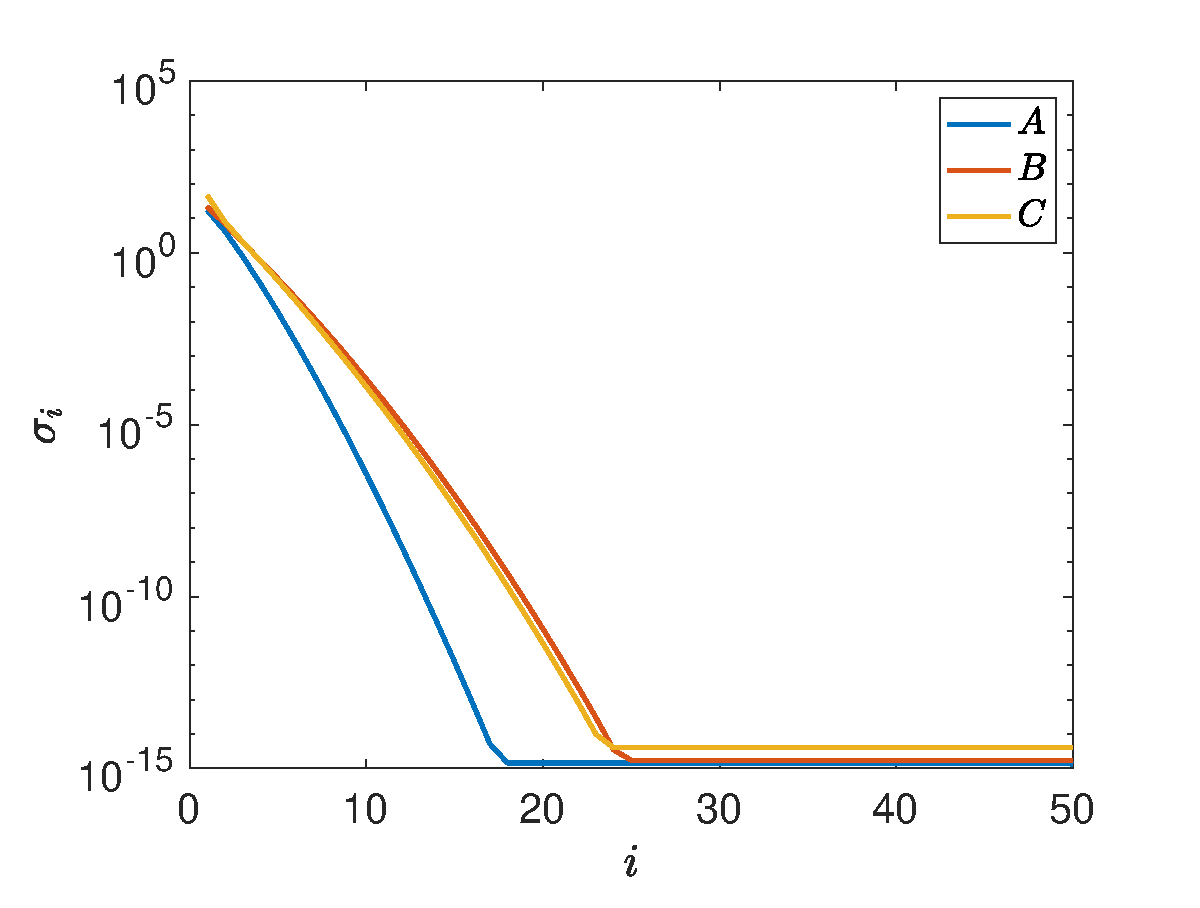
\includegraphics[height=6cm]{./decay_sing_vals.eps}
	\caption{Decay of the singular values $\sigma_i$ for increasing $i$ using $M=N=5$.}
	\label{fig:decay_sigma}
\end{figure}%
\\
We can now check the correctness of our method. We consider first $M=1,N=2$ to keep the sizes controlled. The low-rank approximations of $\mathbf{A},\mathbf{B}$ are obtained from their SVDs after truncating the singular values lower than $\epsilon=10^{-4}$. For the Hadamard product $\mathbf{C}=\hadamard{A}{B}$, we run Lanczos and \textsc{Matlab} \texttt{svd} routine to get the low-rank approximations we need. We select a tolerance of $\epsilon^2$, a maximum number of iteration of $10^3$ and the matrix $\mathbf{C} \mathbf{C}^T$.
A visual comparison of the singular values gets
\begin{align}
	\diag(\mathbf{\Sigma}_{Lan})&=(4.65e+01, \  7.36e+00, \  1.34e+00, \  2.08e-01, \  2.75e-02, \  3.08e-03, \  2.90e-04, \  1.93e-06)^T, \\
	\diag(\mathbf{\Sigma}_{svd})&=(4.65e+01, \  7.36e+00, \  1.34e+00, \  2.08e-01, \  2.75e-02, \  3.12e-03, \    2.97e-04)^T.
\end{align}
and qualitatively validates our method. A similar comparison holds for the singular vectors. A more quantitative analysis looks at the Frobenius norms of the resulting matrices, and gives
\begin{align}
	\norm{(\mathbf{U}_A\mathbf{\Sigma}_A\mathbf{V}_A^T)\star(\mathbf{U}_B\mathbf{\Sigma}_B\mathbf{V}_B^T)-\mathbf{U}_{Lan}\mathbf{\Sigma}_{Lan}\mathbf{V}_{Lan}^T}_F&=2.9135e-06, \\
	\norm{\hadamard{A}{B}-\mathbf{U}_{Lan}\mathbf{\Sigma}_{Lan}\mathbf{V}_{Lan}^T}_F&=6.8986e-05, \\
	\norm{(\mathbf{U}_A\mathbf{\Sigma}_A\mathbf{V}_A^T)\star(\mathbf{U}_B\mathbf{\Sigma}_B\mathbf{V}_B^T)-\mathbf{U}_{svd}\mathbf{\Sigma}_{svd}\mathbf{V}_{svd}^T}_F&=6.7492e-05, \\
	\norm{\hadamard{A}{B}-\mathbf{U}_{svd}\mathbf{\Sigma}_{svd}\mathbf{V}_{svd}^T}_F&=2.2818e-05, \\
	\norm{\mathbf{U}_{Lan}\mathbf{\Sigma}_{Lan}\mathbf{V}_{Lan}^T-\mathbf{U}_{svd}\mathbf{\Sigma}_{svd}\mathbf{V}_{svd}^T}_F&=6.7434e-05.
\end{align}
All errors are relatively small, with no significant differences between our implementation and the \texttt{svd} routine. It is also interesting to compare the size $k_A k_B$ of $\mathbf{\Sigma}_A \otimes \mathbf{\Sigma}_B $ and the ones of $\mathbf{\Sigma}_{Lan}$, $\mathbf{\Sigma}_{svd}$, denoted by $k=k_{Lan}$ and $k_{svd}$. We get 
\begin{equation}
	k_A=5, \quad k_B=7, \quad k=k_{Lan}=8, \quad k_{svd}=7.
\end{equation}
Firstly, the result is consistent with the behavior of the singular vectors observed in \figref{fig:decay_sigma}. Secondly, the difference with the standard \texttt{svd} implementation is of just one singular value, coherently with the similar error norms we computed. Thirdly, it confirms the fact that \eqref{eqn:LR_C} does not encode the low-rank properties of the Hadamard product. Indeed, the resulting size of $\mathbf{\Sigma}_A \otimes \mathbf{\Sigma}_B$ is $k_Ak_B=35$, which is much larger compared to $k=8$. In terms of order of magnitude, we have that $k_Ak_B=\mathcal{O}(k^2)$, so that product of low-rank approximations drastically increases the ranks, and the good compression properties cannot be captured. \\
In order to test the computational advantages of our method, we let $M=N$ vary from $50$ to $300$. The other parameters are not changed from the previous simulation. Since we deal with square matrices, we expect no significant differences if $\mathbf{C} \mathbf{C}^T$ or $\mathbf{C}^T \mathbf{C}$ is used. However, we decide to verify it, with the two approaches named \textit{Lanczos 1} and \textit{Lanczos 2} respectively.
We check the correctness of our results by computing the error norms. \figref{fig:errors} reports 	$\norm{(\mathbf{U}_A\mathbf{\Sigma}_A\mathbf{V}_A^T)\star(\mathbf{U}_B\mathbf{\Sigma}_B\mathbf{V}_B^T)-\mathbf{U}_{Lan}\mathbf{\Sigma}_{Lan}\mathbf{V}_{Lan}^T}_F$ for different values of $N$, comparing them with the \texttt{svd} routine. The order of magnitude is the same, with a minor preference for the first version of the Lanczos method. 
\begin{figure}[htbp]
	\centering
	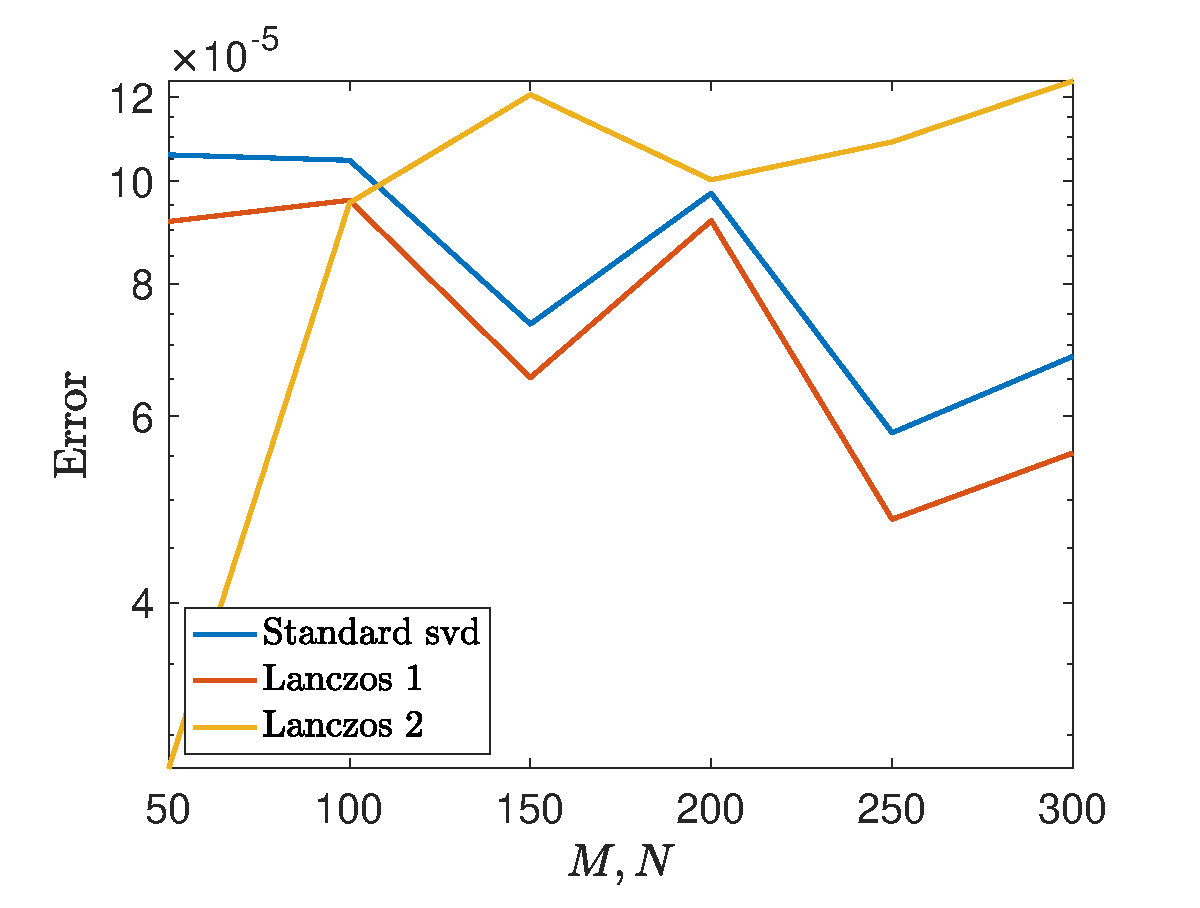
\includegraphics[height=6cm]{./error.eps}
	\caption{Error norms $\norm{(\mathbf{U}_A\mathbf{\Sigma}_A\mathbf{V}_A^T)\star(\mathbf{U}_B\mathbf{\Sigma}_B\mathbf{V}_B^T)-\mathbf{U}_{Lan}\mathbf{\Sigma}_{Lan}\mathbf{V}_{Lan}^T}_F$ with Lanczos method and $\norm{(\mathbf{U}_A\mathbf{\Sigma}_A\mathbf{V}_A^T)\star(\mathbf{U}_B\mathbf{\Sigma}_B\mathbf{V}_B^T)-\mathbf{U}_{svd}\mathbf{\Sigma}_{svd}\mathbf{V}_{svd}^T}_F$ with the \texttt{svd} routine as a function of $N=M$.}
	\label{fig:errors}
\end{figure}%
We also measure the execution time, with the results reported in \figref{fig:time}. For small matrices, \texttt{svd} is preferred over our approach. This is possibly due to \textsc{Matlab} optimizations triggered for small sizes. The in-built algorithm is probably different from a simple implementation of Lanczos method, and outperforms our approach, at least in terms of execution times. We also recall that the matrix-vector multiplication we proposed in Section \ref{sec:matvec_hadamard} becomes effective when $k_A^2/n \simeq k_B^2/n<1$ and $n$ is sufficiently large. Since for small matrices the ratios are not significantly less than one, the benefits of our approach are not evident. Increasing the sizes, important differences appear. The speedup factor we get is almost $10$ compared to the standard \texttt{svd} implementation, and our approach should be preferred.
\begin{figure}[htbp]
	\centering
	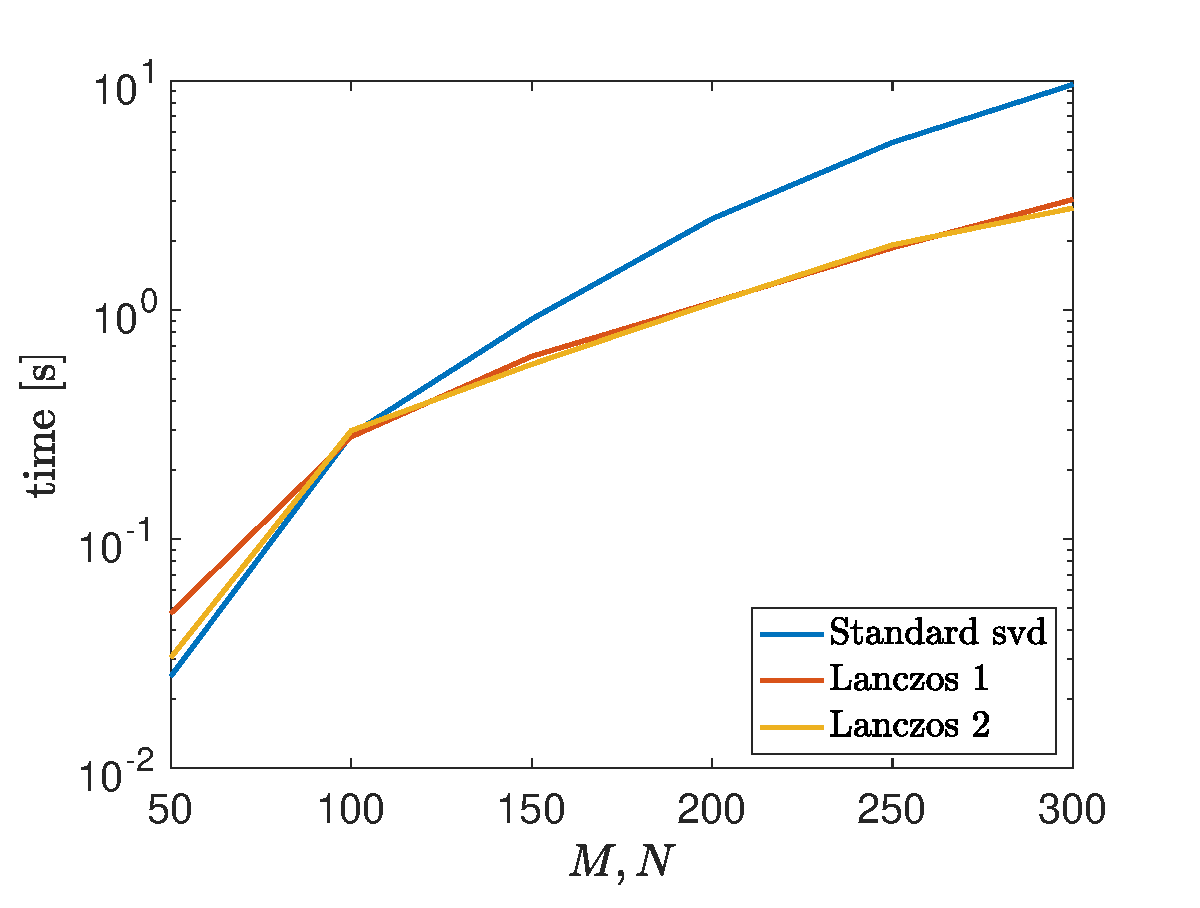
\includegraphics[height=6cm]{./time.eps}
	\caption{Execution time of the Lanczos method and \textsc{Matlab} routine \texttt{svd} to extract the low-rank approximation of $\mathbf{C}$ as a function of $N=M$.}
	\label{fig:time}
\end{figure}%
Finally, we analyze the compression properties of the Hadamard product. Using \eqref{eqn:LR_C}, we get a matrix with size $k_Ak_B$, while Lanczos methods keeps only $k$ vectors. From \figref{fig:dimension}, it is evident that $\mathbf{\Sigma}_A \otimes \mathbf{\Sigma}_B$ does not efficiently encode the low-rank structure of the Hadamard product. In particular, a trend $k_Ak_B=\mathcal{O}(k^2)$ can be observed. The differences with standard \textsc{Matlab} implementation are rather minimal.
\begin{figure}[htbp]
	\centering
	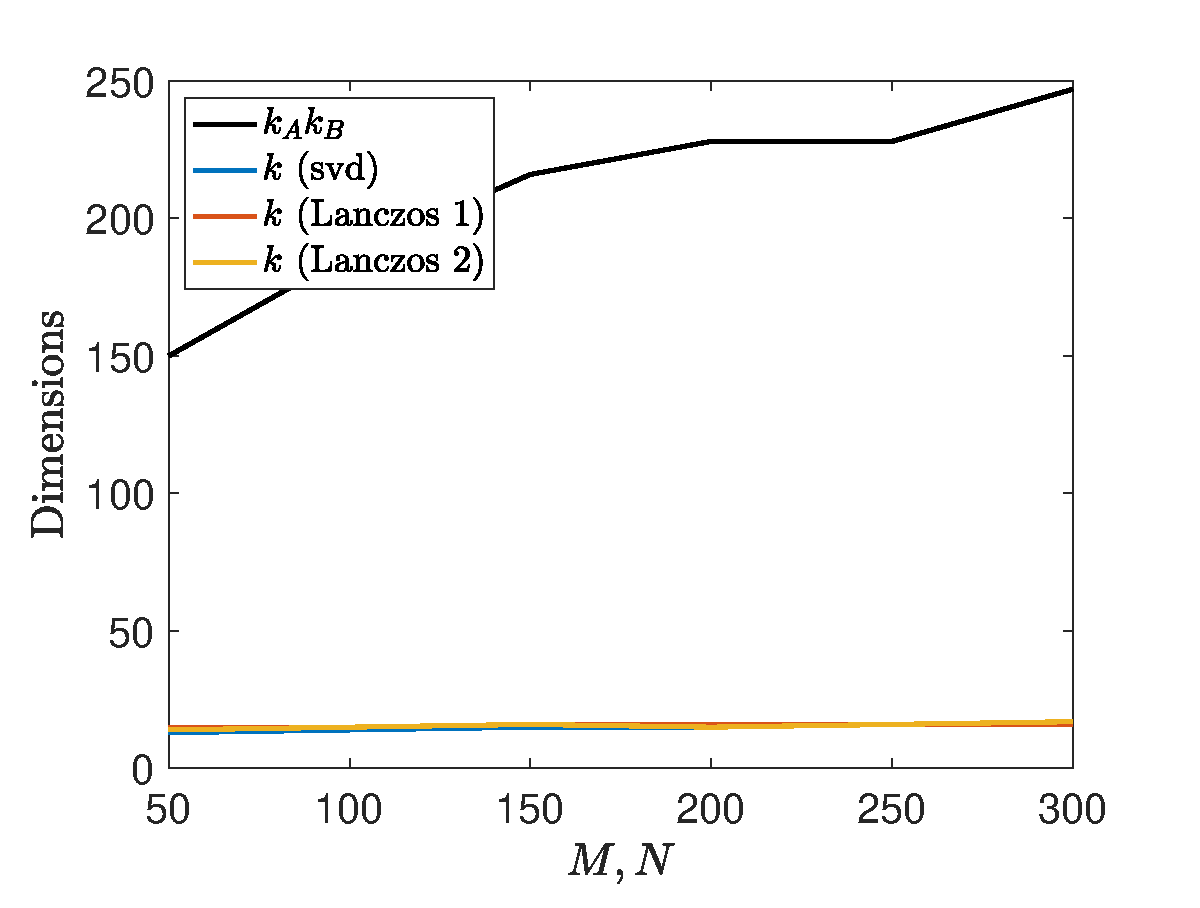
\includegraphics[height=6cm]{./dimension.eps}
	\caption{Size $k_Ak_B$ of $\mathbf{\Sigma}_A \otimes \mathbf{\Sigma}_B$, size $k$ of $\mathbf{\Sigma}_{Lan}$ obtained via Lanczos method and size of $\mathbf{\Sigma}_{svd}$ obtained via \textsc{Matlab} routine \texttt{svd} as a function of $N=M$.}
	\label{fig:dimension}
\end{figure}% 
\\
As a side remark, we point out that the starting guess $\mathbf{u}_1$ for Lanczos method is selected randomly. Even though the results are quite robust with respect to such a variability, a slightly different computational performance can be expected at each run of the algorithm. \\
Finally, the selected tolerance $\epsilon^2$ in Lanczos method can be further decreased to get better approximations, even though errors due to machine precision will eventually play a significant role.  

\section{Conclusion}
In this project we studied the low-rank approximation properties of the element-wise product of two matrices. It is known that the Hadamard product generally multiplies ranks, so that compression properties can be lost, even though the starting matrices are compressed efficiently. However, exploiting a suitable representation, we presented a method able to efficiently compress the resulting matrix via its singular value decomposition. It uses the well-known Lanczos method to compute eigenpairs, taking advantage from a fast matrix-vector multiplication. As a practical application of the method, we considered the low-rank approximation of the product of bi-variate functions on a tensorial grid. We showed that our method gives an error similar to standard approaches, while obtaining a significant speedup for large matrices.



\begin{thebibliography}{}
	\bibitem{Schneider} R. Schneider, A. Uschmajew. Approximation rates for the hierarchical tensor format in periodic Sobolev spaces. \textit{J. Complexity}, 2014.
	\bibitem{Perisa} D. Kressner, L. Periša. Recompression of Hadamard Products of Tensor in Tucker Format. \textit{SIAM Journal on Scientific Computing}, 2017.
	\bibitem{Simon} H. D. Simon, H. Zha. Low-rank Matrix Approximation using the Lanczos Bidiagonalization Process with Application. \textit{SIAM Journal on Scientific Computing}, 2000.
	\bibitem{Quarteroni} A. Quarteroni, R. Sacco, F. Saleri. Numerical Mathematics. \textit{Springer}. 2007.
	\bibitem{Massei} S. Massei, L. Periša. Lecture notes for the EPFL course Computational Linear Algebra. 2019.
\end{thebibliography}




\end{document}  




